\documentclass{UoYCSproject}
\usepackage[backend=biber]{biblatex}
\usepackage{graphicx}
\usepackage{float}
\addbibresource{references.bib}
\author{Sophie Wood}
\title{Model-driven software migration between microcontrollers}
\date{Version 0.1, 2018-May-16}
\supervisor{Simos Gerasimou}
\SWE
% TODO update wordcount
\wordcount{0}

% TODO update includes/excludes
\includes{Appendices TODO}

\excludes{TODO}

% TODO update abstract
\abstract{TODO}

% TODO update acknowledgements
\acknowledgements{TODO}

\begin{document}
\maketitle
\listoffigures
\listoftables

\chapter{Introduction}
\section{Background and Motivation}

Bartels et al. define obsolescence as ``materials, parts, devices, software, services and processes that become non-procurable from their original manufacturer or supplier'' \parencite{bartels2012strategies}. Both software and hardware can be subject to obsolescence problems. 

Issues with hardware obsolescence have been driven by the growth of the electronics industry. This has reduced the life cycle of electronic parts as competitors release products with better functionality and features. Existing products are no longer commercially viable and therefore go out of production \parencite{bartels2012strategies}. This is a particular issue in the defence/aerospace sectors as the typical life cycle of a system is 20-30 years or longer \parencite{rojo2010obsolescence}. As such, parts will become unavailable before the system is completed. Singh et al. found that these systems ``often encounter obsolescence problems before they are fielded and always during their support life'' \parencite{singh2006obsolescence}.

Obsolescence is also a concern in the software industry. Businesses must continuously update their products in order to stay ahead. Bill Gates has said: 
\begin{quote}
``The only big companies that succeed will be those that obsolete their own products before someone else does.'' \parencite{bartels2012strategies}
\end{quote}
There are three main causes of software obsolescence \parencite{sandborn2007obsolescence}:
\begin{description}
\item[(1) Logistical:] digital media obsolescence, formatting, or degradation limits or terminates access to software
\item[(2) Functional:] hardware, requirements, or other software changes to the system obsolete the functionality of the software
\item[(3) Technological:]  the sales and/or support for commercial off the shelf (COTS) software terminates
\end{description}
A particular issue is that hardware obsolescence can drive software obsolescence and vice versa. Software obsolescence can also be caused by lack of skills. For example, there may be a limited number of people that are competent in the language the system is written in. If these people leave the company, the system can no longer be maintained \parencite{rajagopal2014software}. 

Again avionics/military and other ``safety-critical'' systems particularly struggle with software obsolescence issues as even small changes may have to go through extensive and costly qualification/certification processes \parencite{singh2006obsolescence}. For example, the US Navy estimates that obsolescence problems can cost up to \$750 million annually \parencite{adams2005getting}. Sandborn and Myers also found that sustainment costs (which include costs related to obsolescence) dominate the system costs in the case of development of an F-16 military aircraft \parencite{sandborn2008designing}. 
 
Strategies for obsolescence mitigation/management have generally focused on hardware obsolescence problems. This is despite software obsolescence costs often equalling or exceeding that of hardware. Proactive measures to mitigate obsolescence (e.g. improving code portability or using open-source software) often require either a large amount of resources or resources that are unavailable. Reactive strategies for tackling obsolescence include software license downgrades (i.e. customers can adapt legacy versions of the software by purchasing a licence for the latest version and applying that to the older product); purchasing the source code and third party support (i.e. a third party will take over maintenance of the legacy software). If these strategies are insufficient, the legacy system may have to be redeveloped or rehosted \parencite{sandborn2007obsolescence}. However, many such software modernisation projects are abandoned or not completed within the planned timescale/budget \parencite{kowalczyk2009model}. 

Model-driven software modernisation (MDSM) is a set of strategies that use model-driven engineering (MDE) to address the above issues by (partially) automating the process of modernisation. These approaches have already proved feasible by Kowalczyk and Kwieci\'nska who demonstrated the modernisation of a project written in Java 1.4 and the Hibernate 2.x framework, which uses XML mappings, into Java 1.5 and Hibernate 3.x which uses Java Persistence API (JPA) annotations \parencite{kowalczyk2009model}. Additionally, a model-driven approach is employed in industry by the Sodifrance company who have migrated a large-scale banking system (at a size of around one million lines of code) to J2EE \parencite{fleurey2007model}.

The Defence Science and Technology Laboratory (DSTL) at the Ministry of Defence (MoD) have identified several instances of software obsolescence they would like to tackle. A problem of particular interest is ``the migration of an entire software system from a legacy hardware platform to a modern more powerful platform'' \parencite{gerasimou2017technical}. This report will explore how MDSM processes can be used to partially automate the migration of code between microprocessors. A case study implementing the migration of code between a Parallax Propeller Activity Board and an Arduino Uno will be used to demonstrate the approach developed.
 
\section{Project Goals}
TODO
\section{Project Scope}
TODO
\section{Report Structure}
TODO

\chapter{Literature Review}
TODO: write introduction to the literature review chapter
\section{Existing Work}
% Approaches to the general problem of software obsolescence
% Approaches to the specific microcontroller problem
\subsection{Obsolescence}
% Summary of all strategies
% Discussion that most of these are not applicable to sw -> but talk about specific tools
% Discuss other strategies/attempts
The paper by Rojo et al. from 2010 summarises the existing literature for tackling obsolescence \parencite{rojo2010obsolescence}. Although they identified many strategies for handling the obsolescence of electronic components, very few methods were relevant for dealing with software obsolescence. However, they conclude that sectors such as the defence industry would benefit from managing this problem.
\newline
They did identify two tools ``se-Fly Fisher'' and ``R2T2'' (Rapid Response Technology Trade) that could be useful for managing software obsolescence. These tools are used for design refresh planning. Design refresh planning deals with obsolescence in a proactive manner by planning the best times for performing a redesign of the system during the sustainment stage of its lifecycle. 
\newline
Se-Fly Fisher uses the technology curves of each part of the system to: forecast how often a system baseline should change; identify replacement resources and estimate the benefit of each system baseline change \parencite{rojo2010obsolescence}.
Similarly, R2T2 can: forecast system obsolescence; allow for comparisons to alternative solutions; produce a life cycle obsolescence plan for the elements that require refreshment and plan when element replacements should occur \parencite{herald2009obsolescence} .

% Pros and cons of these tools
% In terms of SW obs.
% Pro - can make sure you e.g. hire people will correct skillset
% Pro - switch to other COTS
% Con - does not deal well if equivalent parts are unavailable -> SW 

\section{Model Driven Engineering}
%TODO: this should be edited to have a stronger relation to the project
Model Driven Engineering (MDE) was developed in order to address complexity within the problem space of computing. In the past, approaches for enabling programmers to develop code more easily have focused on simplifying the solution space. This was achieved by providing abstractions such as higher-level programming languages or providing operating systems to manage the difficulty of programming hardware directly. However, these solutions are unable to express domain concepts effectively, unlike MDE techniques \parencite{schmidt2006model}. Furthermore, it has been found that MDE can also be utilised in automating the software development process \parencite{bezivin2004search}.
\newline
The rest of this section introduces the terminology and main components of MDE.

\subsection{Domain-Specific Modelling Languages (DSMLs)}
Meta-meta-modelling mechanisms such as the Object Management Group's (OMG) Meta Object Facility (MOF) can be used to create modelling languages for a given problem domain \parencite{mussbacher2014relevance}. The key components of the OMG's approach to DSMLs are \parencite{bezivin2001towards}:
\begin{description}
\item[Models:] A model is a simplification of a system built with an intended goal in mind. Models should be easier to use than the original system. This is achieved by abstracting out details of the system that are unnecessary for the target model's intended purpose.
\item[Meta-models:] A meta-model is the explicit specification of an abstraction (i.e. model). 
\item[Meta-meta-models:]  A meta-meta-model is used to define meta-models. In particular, the OMG define the MOF (Meta Object Facility) which is a self-defined meta-meta-model.
\end{description}

% TODO: insert figure of MDA layers?

\subsection{Model Transformations}
There are three main categories of model transformation:
\begin{description}
\item[Model-to-model (M2M):] M2M transformations are used to translate source models to target models. The source and target models can be instances of the same or different meta-models \parencite{czarnecki2003classification}.
\item[Model-to-Text (M2T):] These can be considered a special case of M2M transformations. It is often the case that M2T transformations are used for code generation. The most common approach to M2T transformation is a template-based approach. A template contains mixtures of static text and dynamic sections that can be used to access information from the source model \parencite{czarnecki2003classification}.
\item[Text-to-Model (T2M):]  T2M transformations can be used to transform code to a model (conforming to a language meta-model). Model discoverer tools such as MoDisco \parencite{bruneliere2014modisco} are the easiest way to perform T2M transformations on code \parencite{kowalczyk2009model}.
\end{description}

\subsection{The Epsilon Framework}
Epsilon is a family of programming languages for model management tasks. It provides (among others) the following languages of interest \parencite{kolovos2010epsilon}:
\begin{description}
\item[Epsilon Object Language (EOL):] EOL is the common basis for the languages provided by Epsilon. It can be used for querying and modifying models.
\item[Epsilon Validation Language (EVL):] EVL is used for model validation.
\item[Epsilon Transformation Language (ETL):] ETL is used for M2M transformations.
\item[Epsilon Generation Language (EGL):] EGL is used for M2T transformations.
\end{description}
Epsilon also enables the use of ANT tasks to create workflows of different tasks (e.g. a validation followed by a
transformation followed by code generation) \parencite{kolovos2010epsilon}.
\newline
Epsilon has been chosen as the framework for this project over others for the following reasons:
\begin{itemize}
\item It is well documented with many tutorials as well as ``The Epsilon Book'' being freely available. Additionally, there is an active forum for any questions not answered by these sources \parencite{epsilonsite}.
\item It is well integrated with Eclipse (for example, syntax/error highlighting is provided in the editor and there are graphical tools for running/debugging programs) and has been an official project since 2006 \parencite{epsilonsite}.
\item Epsilon provides a connectivity layer (EMC). This layer allows EOL programs to access models of different modelling technologies including Eclipse Modelling Framework (EMF) models and XML documents \parencite{epsilonsite}.
\item I am already familiar with how to use the framework.
\end{itemize}

\section{Microcontroller Background}
The project involves migration of code from a Parallax Propeller Activity Board to an Arduino Uno. However, since some features of the boards are different, this must be taken into account when migrating code. For example, the Propeller Activity Board uses an 8-core microcontroller whereas the Arduino Uno only has a single core. This must be taken into account during the code migration process. The following section discusses the important features and differences between the two boards.

\subsection{Parallax Propeller Activity Board}
\begin{figure}[H]
  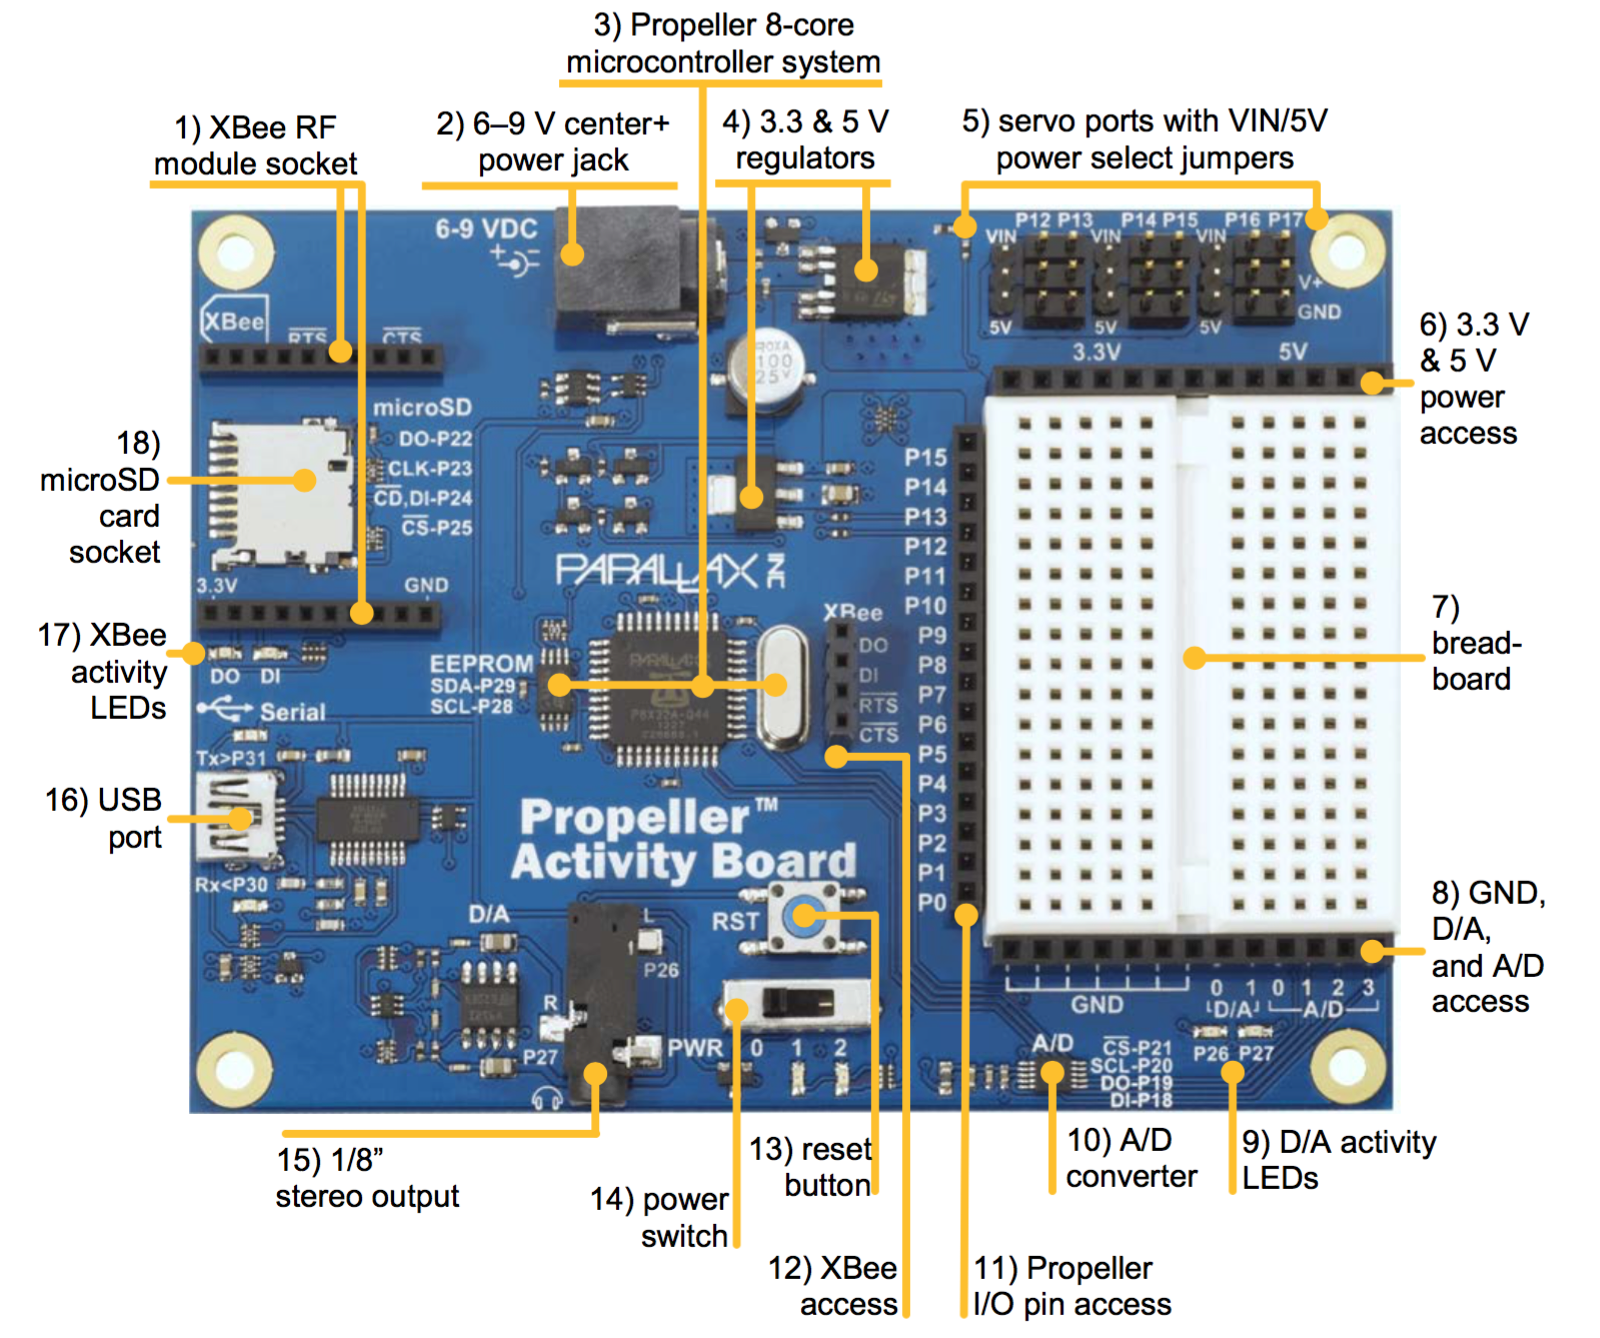
\includegraphics[width=\linewidth]{graphics/propeller_board.png}
  \caption{Features of the Parallax Propeller Activity Board \parencite{propellerspec}.}
  \label{fig:prop_board}
\end{figure}

The key features of the Parallax Propeller Activity Board are \parencite{propellerspec}:
\begin{itemize}
\item Built-in 8-core Propeller P8X32A microcontroller
\item 64KB EEPROM
\item XBee wireless module socket
\item 16 digital I/O pins
\item 4 Analog-to-Digital pins
\item 2 Digital-to-Analog pins
\end{itemize}

\subsection{Arduino Uno}
%TODO: figure out which version I will be using
\begin{figure}[H]
  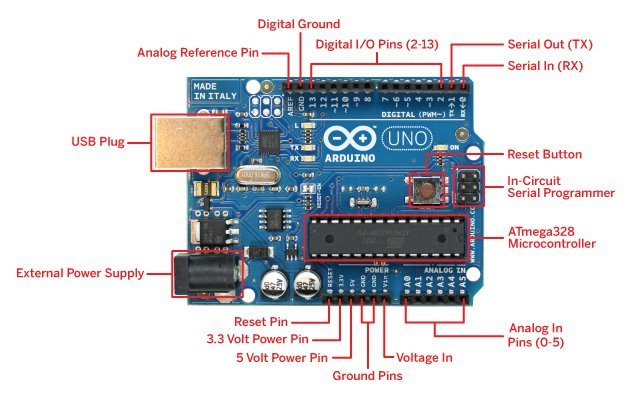
\includegraphics[width=\linewidth]{graphics/arduino_board.jpg}
  \caption{Features of the Arduino Uno \parencite{arduinodiagram}.}
  \label{fig:arduino_uno}
\end{figure}

The key features of the Arduino Uno are \parencite{arduinospec}:
\begin{itemize}
\item Built-in single-core ATmega328 microcontroller
\item 32KB flash memory
\item 2KB SRAM
\item 1KB EEPROM
\item 14 digital I/O pins (6 provide PWM output)
\item 6 analog input pins
\end{itemize}


\section{Tools}

\chapter{Methodology}
%TODO

\chapter{Requirements}
%TODO

\chapter{Design and Implementation}
%TODO

\chapter{Evaluation}
%TODO

\chapter{Conclusion}
%TODO

\printbibliography
\end{document}